\documentclass[12pt]{article}
\usepackage{amsmath}
\usepackage{times}
\usepackage{graphicx}
\usepackage{color}
\usepackage{multirow}
%
\usepackage[authoryear]{natbib}
%
\usepackage{rotating}
\usepackage{bbm}
\usepackage{latexsym}
%\DeclareGraphicsExtensions{.eps,.png}

% reference links
\usepackage{nameref,hyperref}
\usepackage[table]{xcolor}
\hypersetup{
    colorlinks = true,                    % text and not border
    citecolor = {teal},
    linkcolor = {purple},
           }
% black, blue, brown, cyan, darkgray, gray, green, lightgray, lime, 
% magenta, olive, orange, pink, purple, red, teal, violet, white, yellow.

%%% margins 
\textheight 23.4cm
\textwidth 14.65cm
\oddsidemargin 0.375in
\evensidemargin 0.375in
\topmargin  -0.55in
%
%\renewcommand{\baselinestretch}{2}
%
\interfootnotelinepenalty=10000
%
\renewcommand{\thesubsubsection}{\arabic{section}.\arabic{subsubsection}}
\newcommand{\myparagraph}[1]{\ \\{\em #1}.\ \ }
\newcommand{\citealtt}[1]{\citeauthor{#1},\citeyear{#1}}
\newcommand{\myycite}[1]{\citep{#1}}

% Different font in captions
\newcommand{\captionfonts}{\normalsize}

\makeatletter  
\long\def\@makecaption#1#2{%
  \vskip\abovecaptionskip
  \sbox\@tempboxa{{\captionfonts #1: #2}}%
  \ifdim \wd\@tempboxa >\hsize
    {\captionfonts #1: #2\par}
  \else
    \hbox to\hsize{\hfil\box\@tempboxa\hfil}%
  \fi
  \vskip\belowcaptionskip}
\makeatother   
%%%%%

\renewcommand{\thefootnote}{\normalsize \arabic{footnote}} 	

\newcommand\norm[1]{\left\lVert#1\right\rVert}

\usepackage{mathtools}
\newcommand{\defeq}{\vcentcolon=}


\begin{document}
\hspace{13.9cm}1

\ \vspace{20mm}\\

{\LARGE\noindent Optimizing individually the variance of the
neural activity regulates the echo-state spectral radius}

\ \\
{\bf \large Fabian Schubert and Claudius Gros}\\
{Institute for Theoretical Physics, Goethe University, Frankfurt a.M., Germany.}\\
%

%\ \\[-2mm]
\noindent
{\bf Keywords:} variance optimization, echo state network, spectral radius, 
biological plausibility, self-organization, universality

\thispagestyle{empty}
\markboth{}{Variance optimization}
%
\ \vspace{-0mm}\\
%
%Abstract
\begin{center} {\bf Abstract} \end{center}
Echo state networks are based on recurrent nets that
provide large selections of non-linear filters of the 
input signal to a perceptron layer. For the echo state 
network to function optimally as a prediction machine, 
the spectral radius $R\!=\!|\Lambda_{max}|$ of the recurrent 
synaptic weight matrix needs to be regulated. This 
implies that the modulus of the largest eigenvalue 
$\Lambda_{max}$ of the synaptic weight matrix should be 
unity, or slightly larger, a condition demanding ostensibly 
a non-local operation. Here we show that $R$ can be 
regulated locally if neurons optimize the variance 
of their own activity. Variance optimization is performed
relative to the variance of the input signal by adapting 
the slope of the transfer function. 

The proposed local adaption rule can be carried out online, 
which implies that it is  biologically plausible and that 
network can react autonomously to changes of the input 
statistics during normal operations. The effectiveness of 
the algorithm is supported by numerical simulations and 
an analytic approximation. The respective optimality 
condition is universal in the sense that it is independent
of the network topology, the link probability and the
distribution of synaptic weights.
%%%%%%%%%%%

%%%%%%%%%%%%%%%%%%%%%%%%%%%%%%%%%%%%%%%%%%%
%%%%%%%%%%%%%%%%%%%%%%%%%%%%%%%%%%%%%%%%%%%

%----------------------------------------
\section{Introduction}
%----------------------------------------

Recurrent network activity may process
time-dependent input signals in at least
two distinct ways. In the first scenario
the network activity is present in the 
absence of a driving input, playing at the
same time a key role in processing input 
signals. The autonomous neural activity may 
be in this case either structured 
\citep{gros2009cognitive,berkes2011spontaneous,mitra2016networks},
or self-organized critical
\citep{petermann2009spontaneous,arviv2015near,cocchi2017criticality}.
Within the second scenario the network becomes active
only when stimulated by sequences of input signals.
Once externally induced, the recurrent activity
provides a reservoir of non-linear transformations
\citep{lukovsevivcius2009reservoir}, both in time
and in space, that may be utilized by a second-state
linear learning unit. One speaks of an echo state
network when the constituting neurons are rate-encoding
\citep{jaeger2005reservoir}, and of a liquid-state
machine for the case of spiking neurons \citep{maass2002real}.

Training the linear output units transform an echo state 
network to an highly effective prediction machine
\citep{ozturk2007analysis,lukovsevivcius2009reservoir},
with the performance needing a fine tuning of the
network properties, in particular the spectral radius
$R=|\Lambda_{max}]$. The activity decays in the absence
of external inputs when the largest eigenvalue 
$\Lambda_{max}$ of the synaptic weight matrix is 
smaller than unity, a precondition for the network
to be able to encode input signals transiently
\citep{yildiz2012re,caluwaerts2013spectral}. Information
is however lost fast when the spectral radius is too fast, 
which is detrimental. A spectral radius of about unit may
is hence best \citep{jaeger2002tutorial}, in the sense 
that it provides a maximal memory capacity
\citep{boedecker2012information,farkavs2016computational}.

A network is said to have the echo-state property when 
a short-term echo, but not a long-term reverberating 
activity, is present in response to a given input
\citep{jaeger2002tutorial}. Echo state networks work
however not in alternating on and off modes, but under
the influence of a continuous stream of input signals,
viz as continuously driven systems. The echo-state property
has hence to be generalized \citep{manjunath2013echo}
in terms of pullback attractors 
\citep{kloeden2000pullback,caraballo2006pullback},
which implies that two nearby internal states converge
under the influence of the same input stream. Optimal
performance in terms of a maximal memory capacity is 
achieved at the edge of chaos, viz at the point when 
the pullback attractor disappears. Here we show that
optimality is attained under the influence of a simple 
and biological plausible self-organizing principle.

Besides their applications as efficient machine learning
algorithms, echo state networks are potentially 
relevant also for information processing in the brain
\citep{nikolic2009distributed,enel2016reservoir}. It
is hence important to examine whether there exist
local and biological plausible principles allowing
to tune the properties of the reservoir to the edge
of chaos \citep{livi2018determination}, in particular 
when a continuous stream of inputs is present. This 
rule needs to be independent of the network topology, 
which is not a locally accessible information, and 
of the distribution of synaptic weights.

\bigskip\bigskip\bigskip\smallskip\noindent

Avalanches in Self-Organized Critical Neural Networks: A
Minimal Model for the Neural SOC Universality Class.
Matthias Rybarsch, Stefan Bornholdt

\bigskip\bigskip\bigskip\smallskip\noindent


\smallskip\noindent
\cite{schuecker2018optimal}
Optimal sequence memory in driven random networks.
{\em
At the transition point, the variance of the recurrent input to
a single unit equals the variance of its own activity.
}

\smallskip\noindent
\citep{wainrib2016local}
A local Echo State Property through the largest Lyapunov exponent.

\smallskip\noindent
\citep{gallicchio2017echo}
Echo state property of deep reservoir computing networks.


\smallskip\noindent
\citep{livi2018determination}
Determination of the edge of criticality in echo state networks 
through Fisher information maximization.

\smallskip\noindent
\citep{boedecker2009initialization}
Initialization and self-organized optimization of recurrent neural network connectivity.

\smallskip\noindent
\citep{gros1990criterion}
Criterion for a good variational wave function (variance optimization).

\smallskip\noindent
\citep{cannon2017stable}
Stable Control of Firing Rate Mean and Variance by Dual Homeostatic Mechanisms.


%----------------------------------------
\section{Regulating the moments of the neural activity}
%----------------------------------------

Rate-encoding neurons come with a set of internal 
parameters, in particular the threshold $b$ and 
the gain $a$. In this study we take $g(z)\!=\!\tanh(z)$
as the transfer function, where the argument is
$z\!=\!a(x\!-\!b)$, with $x$ being equivalent to the 
membrane potential. Neurons adapting on
their own dispose of individual gains
$a_i$ and threshold $b_i$. The time 
evolution of a network characterized by
a recurrent weight matrix $w_{ij}$ is then
%
\begin{equation}
y_i(t+1)=g(a_i(x_i(t)-b_i)),
\qquad\quad
x_i(t)= \sum_{j=1}^N w_{ij}y_j(t)+ E_i(t)
\qquad\quad 
\label{y_t_plus_one}
\end{equation}
%
where $N$ is the number of reservoir neurons. Time 
is discrete and indexed by $t\!=\!0,1,..\,$. For 
the external input $E_i(t)$ we use normal
distributed white noise, with zero mean
and standard deviation $\sigma_{\rm ext}$.

In (\ref{y_t_plus_one}) we have refrained from 
introducing a separate set of input units 
and a matrix linking the inputs to the reservoir
neurons, lumping the statistical effect of the
external driving into a scalar quantity, $E_i(t)$.
For the internal connections $w_{ij}$ we 
selected a connection probability $p\!=\!0.1$.
The magnitude of the non-zero elements of
$w_{ij}$ are drawn then from a normal distribution
with zero mean and standard deviation
$\sigma_{\rm w}/\sqrt{pN}$, a scaling that ensures
that the variance of the two contributions
a neuron receives, external and recurrent,
are of the same order of magnitude \citep{sompolinsky1988chaos}. 
Typically we use $\sigma_{\rm w}\!=\!1.0$.

The value of internal neural parameters needs to be regulated 
on the basis of homeostatic principles 
\citep{marder2006variability}, a mechanism also termed 
intrinsic adaption \citep{triesch2005gradient}. 
Here we propose that the two basic parameters,
the threshold $b_i$ and the gain $a_i$, have
well defined and distinct roles in regulating
the activity, with $b_i\!=\!b_i(t)$ and $a_i\!=\!a_i(t)$ 
being respectively responsible for setting the mean 
and the variance of the neural firing rate.
The adaption rules 
$a_i(t\!+\!1)\!=\!a_i(t)\!+\!\Delta a_i(t)$ and
$b_i(t\!+\!1)\!=\!b_i(t)\!+\!\Delta b_i(t)$
implementing this principle are
%
\begin{equation}
\Delta a_i = \epsilon_{\rm a}\left(\sigma_t^2-(y_i(t)-\bar{y}_i)^2\right),
\qquad\quad
\Delta b_i = \epsilon_{\rm b}\big(y_i(t)-y_t\big)\,
\label{dot_a_b}
\end{equation}
%
where we have denoted the target values for the average and 
for the variance of the neural activity $y_i(t)$ respective
by $y_{\rm t}$ and $\sigma_{\rm t}^2$. An average over extended time scales
are implicitly performed when the update rates 
$\epsilon_{\rm a}$ and $\epsilon_{\rm b}$ are small. 
The trailing average $\bar{y}_i$ showing up in (\ref{dot_a_b}) 
is defined here via
%
\begin{equation}
\bar{y}_i(t+1)\!=\!\bar{y}_i(t)+\bar{\epsilon}\,(y_i(t)-\bar{y}_i(t))\,,
\label{y_trailing}
\end{equation}
%
where $\bar{\epsilon}\ll1$.

%----------------------------------------
\subsection{Spectral radius renormalization}
%----------------------------------------

Echo state networks take their name from the absence
of a long-lasting echo, namely that the transient
stimulation of the network by an external stimulus
evokes an exponentially decaying response. For an
isolated system this condition, the echo state
condition, implies that the fixpoint corresponding
to an inactive network should be stable, namely
that the spectral radius $R=|\Lambda_{max}|$ of 
the rescaled weight matrix should be smaller than unity.
Note that this condition is local in time
\citep{wernecke2019chaos}. With the gain $a_i$ 
multiplying the afferent synaptic weights,
%
\begin{equation}
z_i=a_i(x_i-b_i)
= a_i\left(\sum_{j=1}^N w_{ij}y_j(t)+ E_i(t)\right)-a_ib_i\,,
\label{z_a_w}
\end{equation}
%
adapting the gain is equivalent is equivalent to adapting
the spectral radius. The key point is, that this can 
be done using locally available information, the 
variance of the neural activity and of the distribution 
of the external input $E_i(t)$. Technically, we
evaluate
%
\begin{equation}
R(\widehat{W}_{\rm a}),
\qquad\quad
(\widehat{W}_{\rm a})_{ij}\!=\!a_i W_{ij},
\label{R_widehat_W}
\end{equation}
%
where $\widehat{W}_a$ it the locally rescaled weight matrix.
This procedure reduces to the standard matrix rescaling
when the differences between the individual gains vanish, 
as it will be the case for large network sizes $N\!\to\!\infty$.

%%%%%%%%%%%%%%%%%%%%%%%%%%%%%%%%%%%%%%%%%%%%%%%%%%%%%%%%
\begin{table}[b]
\caption{The parameters used, where $N$ is the network size, 
$p$ is the connection probability of the recurrent weight 
matrix and $\sigma_{\rm w}$ the scale of the standard deviation 
$\sigma_{\rm w}/\sqrt{pN}$, of the $w_{ij}$, compare (\ref{dot_a_b}). 
Further listed are $\epsilon_{\rm a}$, $\epsilon_{\rm b}$ $\bar{\epsilon}$, 
the update rates for the gain, the threshold and the trailing 
average, and the target neural activity, $y_{\rm t}$.
}
\centering
\def\arraystretch{1.3}
\vspace{5pt}
\begin{tabular}{ c | c | c | c | c | c | c }
$N$ & $p$ & $\sigma_{\rm w}$ & $\epsilon_{\rm b}$ & $\epsilon_{\rm a}$ & 
$\bar{\epsilon}$ & $y_{\rm t}$ \\
\hline
\hline
1000 & 0.1 & 1.0 & $2\cdot 10^{-4}$ & $10^{-3}$ & $10^{-4}$ & 0 
\end{tabular}
\label{tableParameters}
\end{table}
%%%%%%%%%%%%%%%%%%%%%%%%%%%%%%%%%%%%%%%%%%%%%%%%%%%%%%%%

%----------------------------------------
\subsection{Variance optimization vs.\ entropy maximization}
%----------------------------------------

The adaption rules (\ref{dot_a_b}) are an abstraction of
the principle of polyhomeostatic optimization \citep{markovic2010self},
which deals with the optimization of entire distribution 
functions. However, instead of maximizing the
entropy \citep{triesch2005gradient}, as for the case
of intrinsic adaption, or minimizing the Fisher information 
\citep{echeveste2014generating}, when deriving self-limiting
Hebbian learning rules, the two leading moments of the
firing rate distribution $\rho(y)$ are regulated. In
order to clarify this relation we consider the case
that one wants to maximize the entropy of the neural
activity under the constraint of a given mean $\mu$
and variance $\sigma^2$. The maximal entropy distributions
is in this case a Gaussian \citep{gros2015complex},
%
\begin{equation}
N_{\mu,\sigma}(y)=\frac{1}{\sqrt{2\pi\sigma^2}}
\mathrm{e}^{-(y-\mu)^2/(2\sigma^2)}
%\propto \mathrm{e}^{\lambda_1 y +\lambda_2y^2}
\,.
\label{Gaussian}
\end{equation}
%

%%%%%%%%%%%%%%%%%%%%%%%%%%%%%%%%%%%%%%%%%%%%
\begin{figure}[t!]
\begin{center}
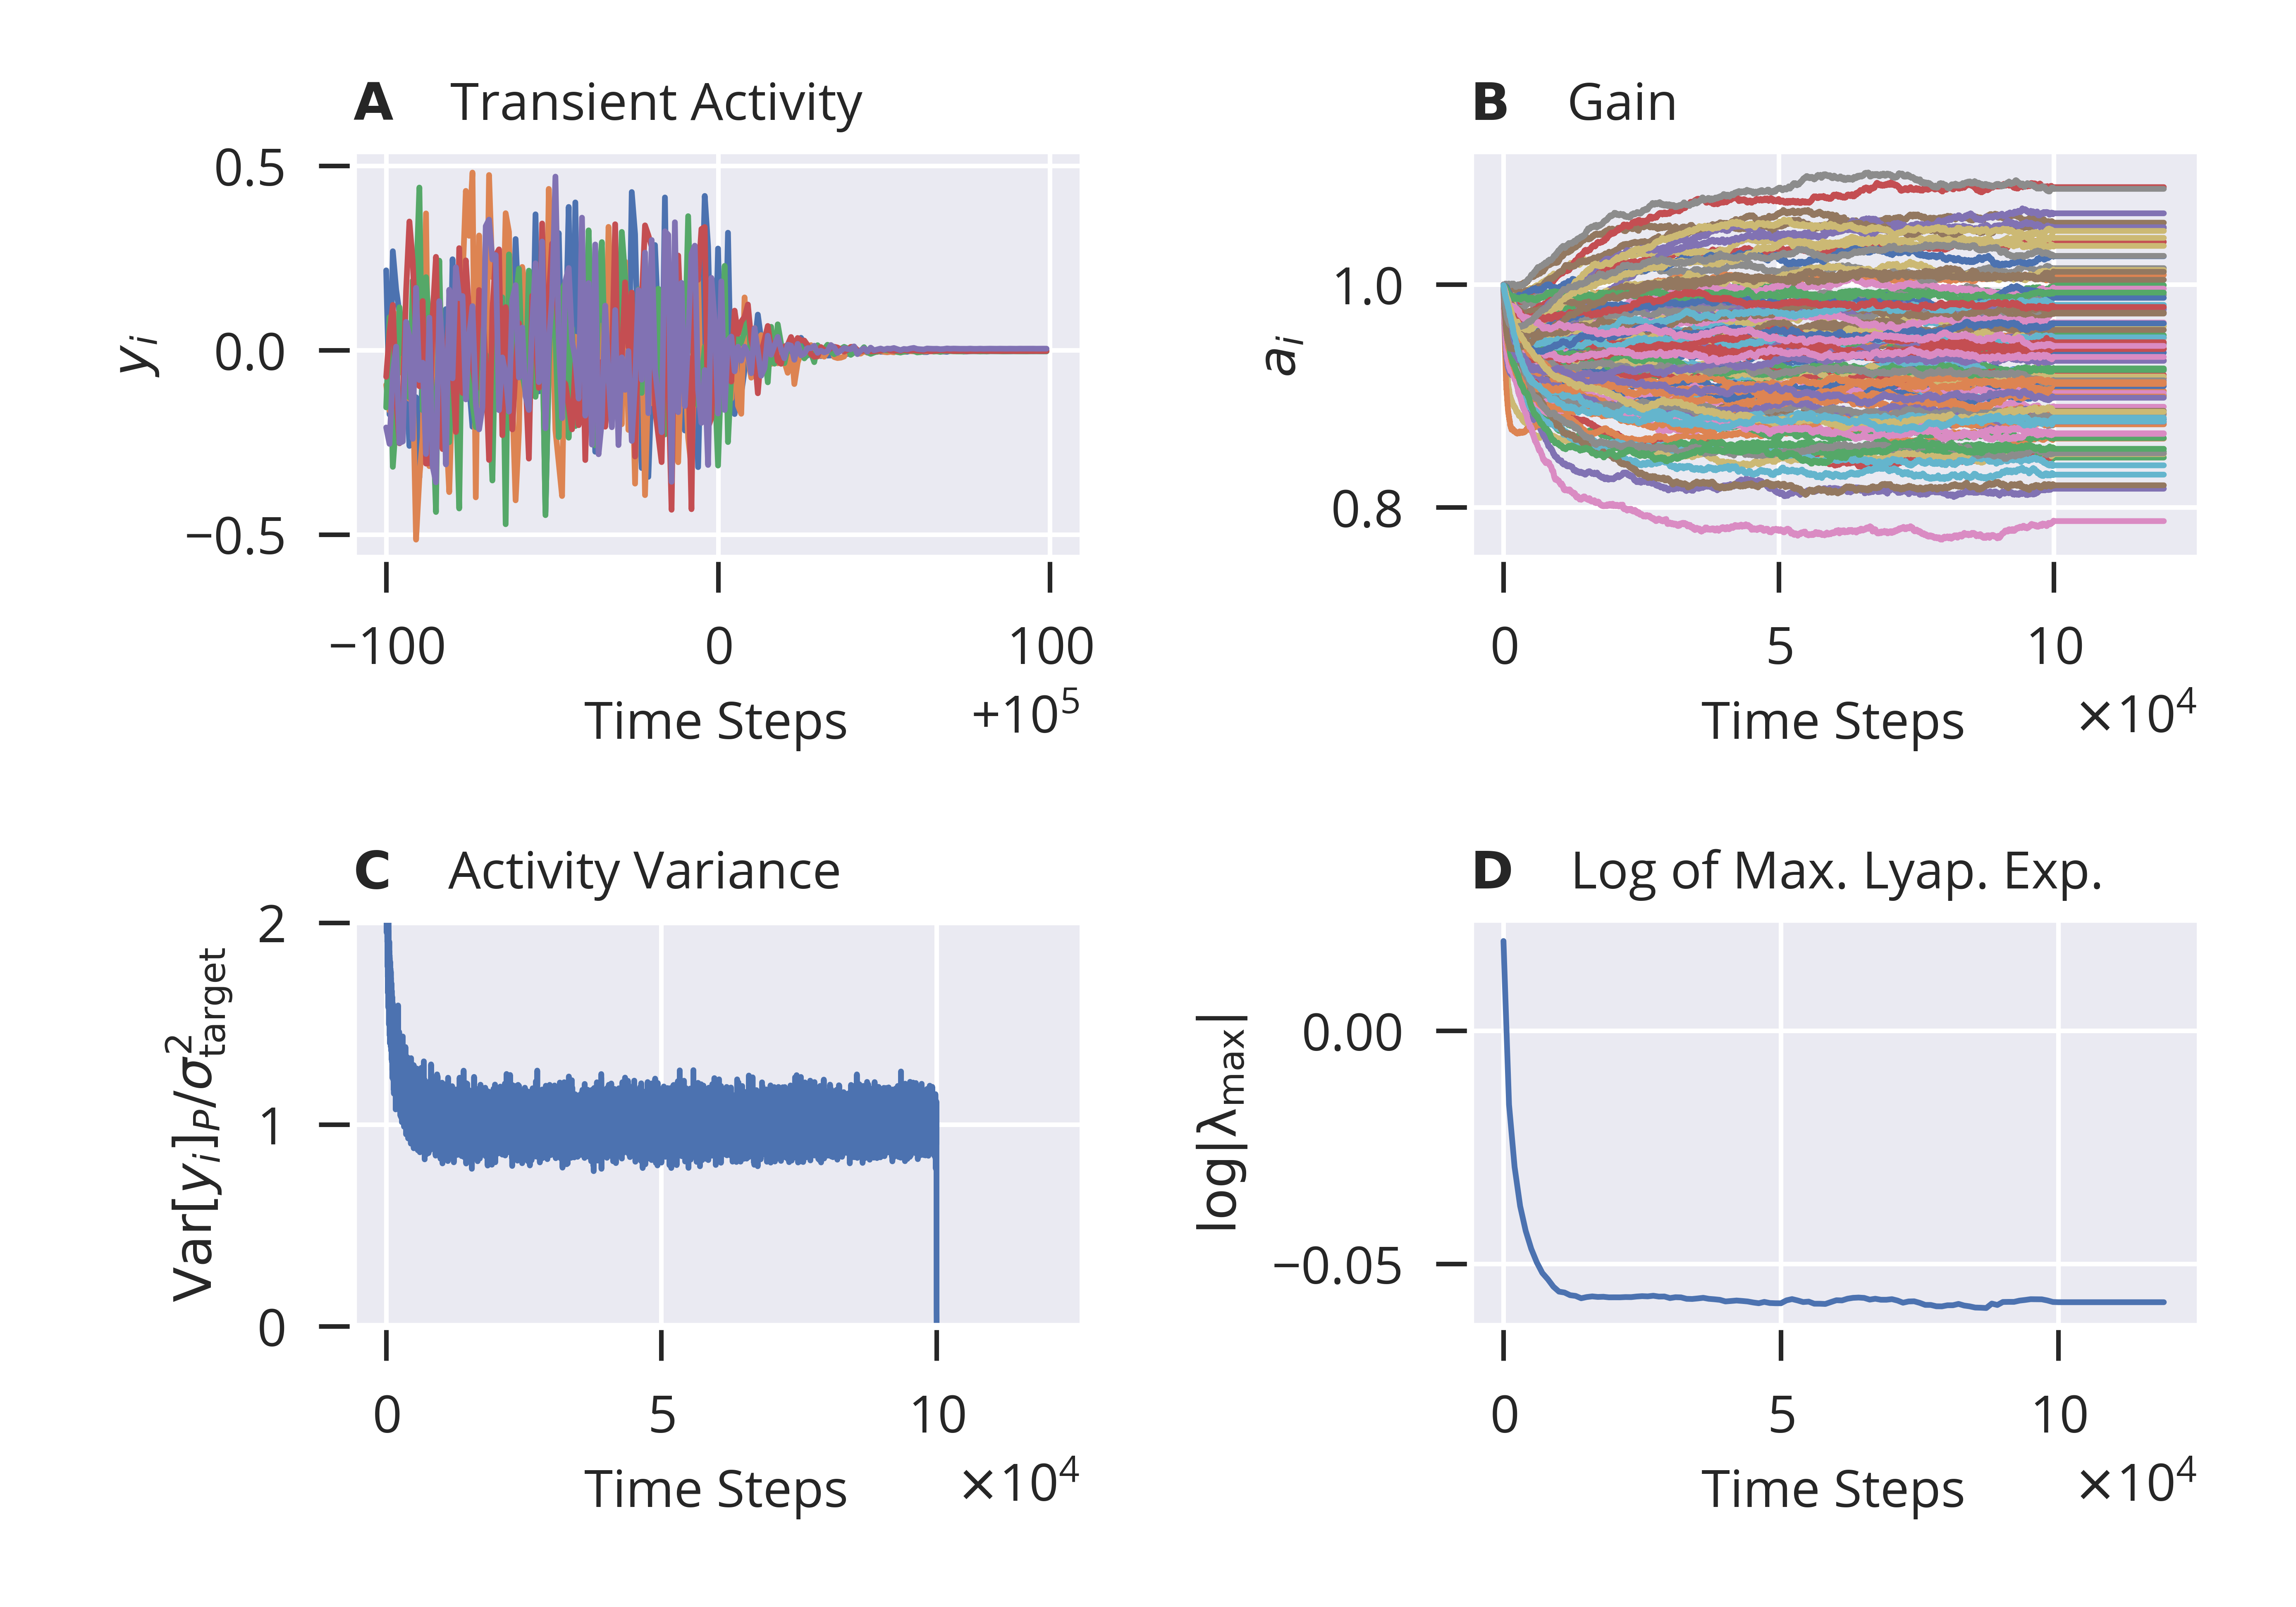
\includegraphics[width=1.0\textwidth]{timeSeries_01.png}
\end{center}
\caption{{\bf Time series.} For $N=1000$ neurons, 
$\sigma_{\rm t}=0.2$, $\sigma_{\rm ext}=0.1$ and the parameters 
given in Table~\ref{tableParameters}, the evolution of 
selected quantities. At $t^E_{\mathrm{off}}=10^5$
the external input is turned off.
{\bf A:} The activity of a random selection of $N/10$ 
neurons, with the activity dying out once the external driving
is absent.
{\bf B:} The evolution of $N/10$ randomly selected 
gains $a_i=a_i(t)$. The individual gains collapse
for large networks, compare Fig.~\ref{Fig:sigma_target_external}.
{\bf C:} The population average of the ratio 
$\sigma^2(y)/\sigma_{\rm t}^2$ between the actual variance 
$\sigma^2(y)=\langle (y_i-\bar{y}_i)^2\rangle/\sigma_{\rm t}^2$
of the neural activity and the target variance $\sigma_{\rm t}^2$.
{\bf D:} The largest Lyapunov exponent
$\log|\Lambda_{max}|$, where $|\Lambda_{max}|$
is the spectral radius and $\Lambda_{max}$
the largest eigenvalue, in magnitude, of the
locally rescaled weight matrix, see (\ref{R_widehat_W}).
}
\label{Fig:timeSeries_01}
\end{figure}
%%%%%%%%%%%%%%%%%%%%%%%%%%%%%%%%%%%%%%%%%%%%

For the neural activity to be close to (\ref{Gaussian})
one needs to minimize the Kullback-Leibler divergence between 
the normal distribution $N_{\mu,\sigma}(y)$ and the actual 
firing rated distribution $\rho(y)$. Doing so, one obtains 
the adaption rules
%
\begin{equation}
\begin{array}{rcll}
\Delta a &=& \epsilon_{\rm a}
    \left(1/a-(x-b)\,\Theta\right)& \\[0.5ex]
\Delta b &=& \epsilon_{\rm b}\, a\,\Theta, &
\Theta= 2y+ (1-y^2)(y-\mu)/\sigma^2
\end{array}\,.
\label{gaussian_Delta_a_b}
\end{equation}
%
Equivalent equations can be derived when considering 
$z\!\to\!ax\!-\!b$ \citep{schrauwen2008improving}, instead
of $z\!=\!a(x\!-\!b)$, as done here, or a sigmoidal transfer 
function \citep{linkerhand2013self}. We note that both
$\Delta a$ and $\Delta b$ are cubic polynomials of $y$, 
even though the objectives, the first two moments of 
$\rho(y)$, involve only linear and quadratic constraints. 
There are several distinct differences between 
(\ref{gaussian_Delta_a_b}) and (\ref{dot_a_b}).
%
\begin{itemize}

\item Despite that $\sigma$ and $\mu$ are the target 
      moments for $\rho(y)$, they are not achieved 
      when the gain and the threshold are adapted under 
      the influence of (\ref{gaussian_Delta_a_b}). This
      is in contrast to (\ref{dot_a_b}), which regulates 
      the moments of $\rho(y)$ closely to their target 
      values, $y_{\rm t}$ and $\sigma_{\rm t}^2$.

\item The adaption rule (\ref{gaussian_Delta_a_b}) are
      inherently stable, due to the fact that they result 
      from minimizing an objective function. The variance
      optimization rules (\ref{dot_a_b}) can however not
      converge when the target values $y_{\rm t}$ and/or 
      $\sigma_{\rm t}$ do not respect that the neural activity 
      $y\!\in\![-1,1]$ is bounded. A $\mu\!>\!1$ would lead 
      f.i.\ to an ever decreasing threshold $b$.
   
\end{itemize}
%%%%%%%%%%%%%%%%%%%%%%%%%%%%%%%%%%%%%%%%%%%%
\begin{figure}[t!]
\begin{center}
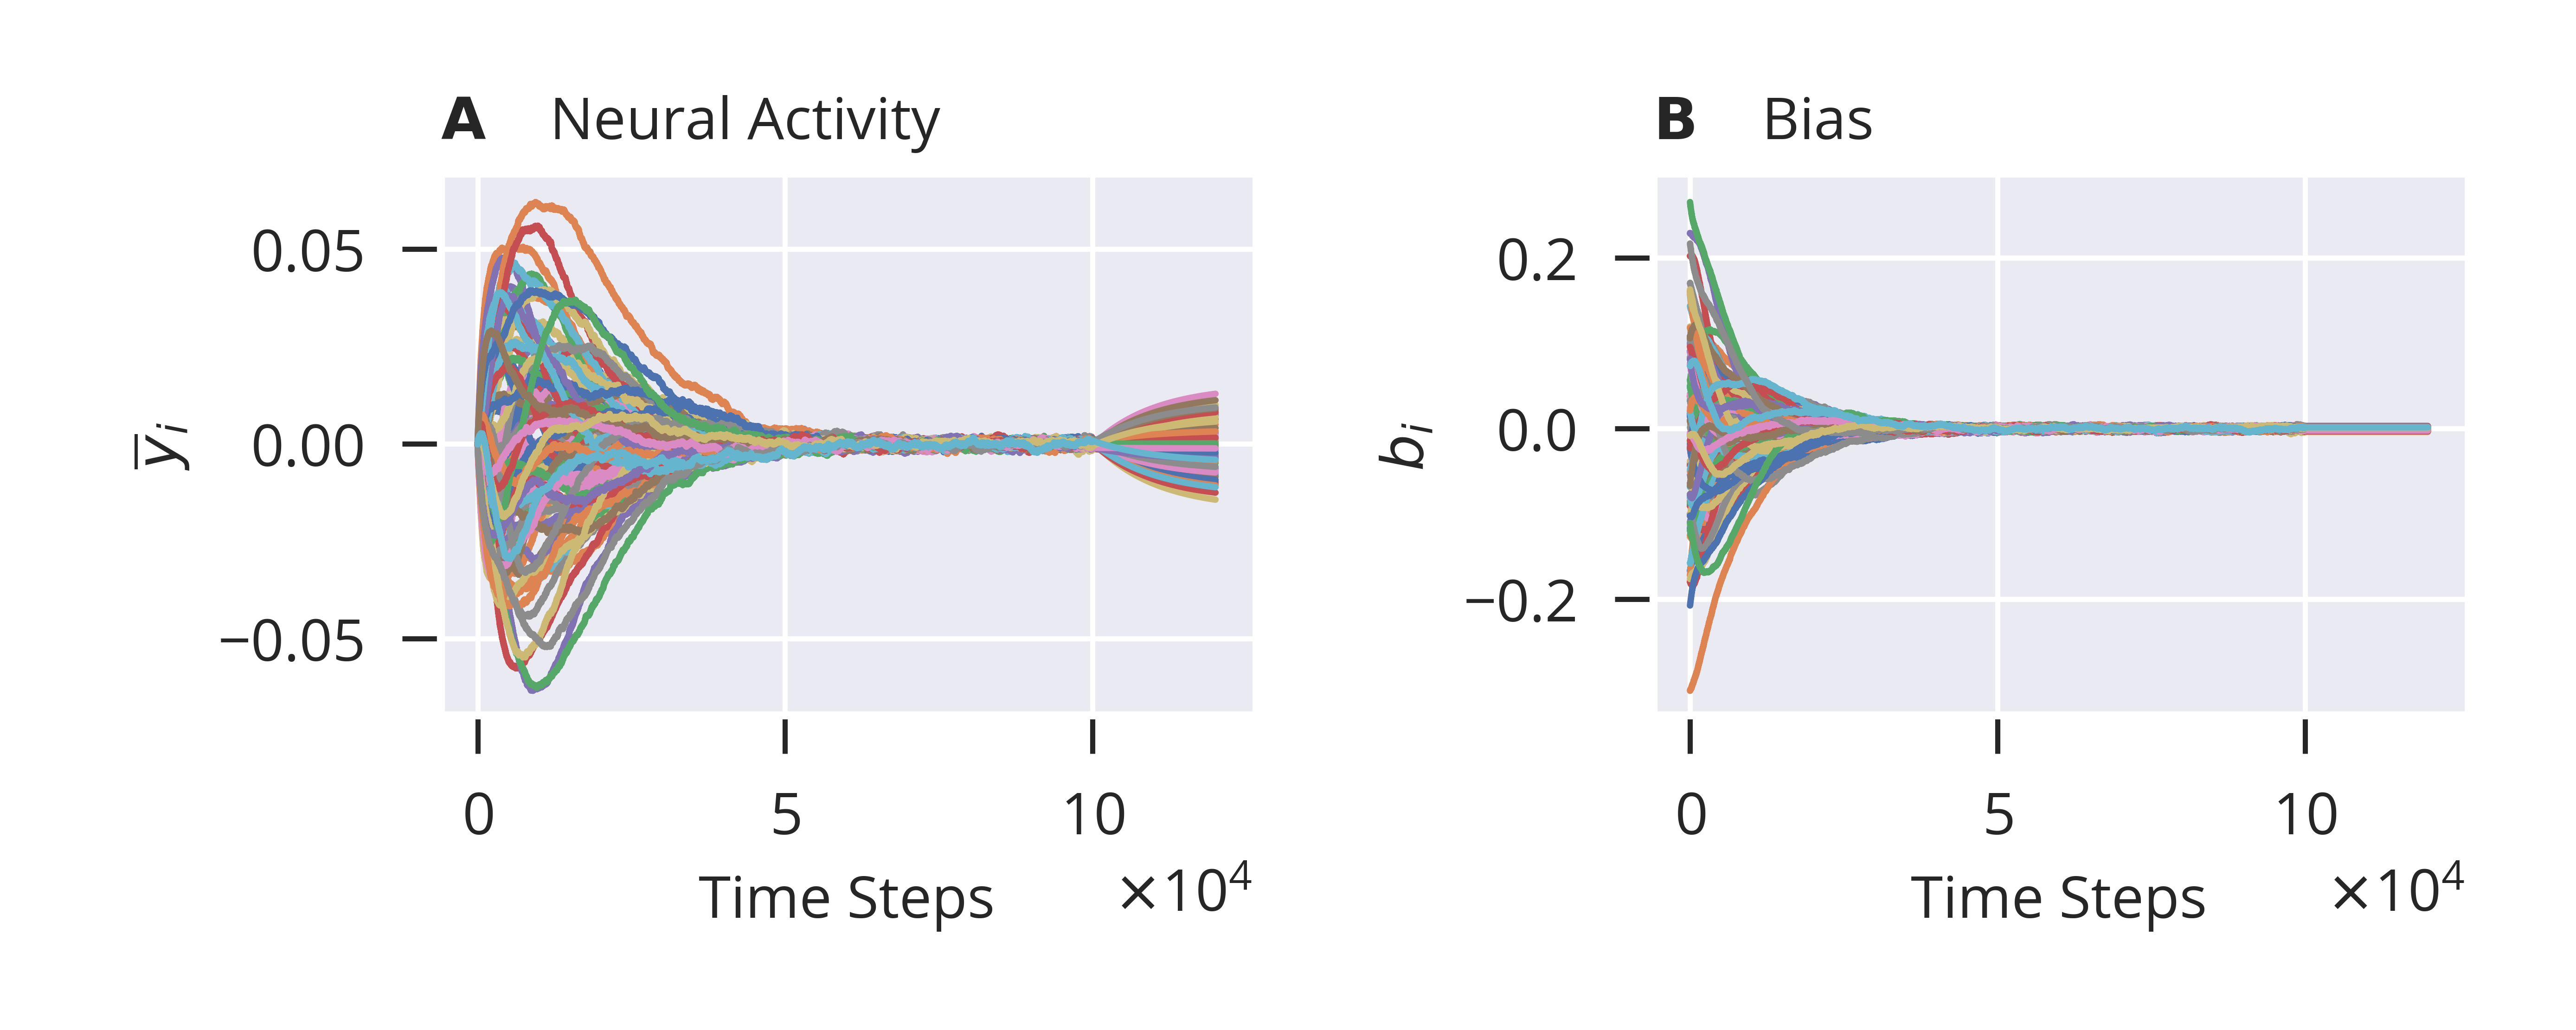
\includegraphics[width=1.0\textwidth]{timeSeries_02.png}
\end{center}
\caption{{\bf Threshold adaption.} Simulation parameters as for
Fig.~\ref{Fig:timeSeries_01}. At $t_{off}=10^5$ the
external input is turned off together with the adaption 
of the the gain and the threshold.
{\bf A:} The trailing average $\bar{y}_i$ of a random selection 
of $N/10$ neurons. The average activity approaches the target 
value $y_{\rm t}=0$, recovering slightly once the external input and 
the adaption of the threshold and the gain is turned off. This
happens because the individual $b_i$ are small but non-zero.
{\bf B:} The evolution of the individual bias $b_i$. The 
stochastic input induces small, barely visible amplitude 
fluctuations.
}
\label{Fig:timeSeries_02}
\end{figure}
%%%%%%%%%%%%%%%%%%%%%%%%%%%%%%%%%%%%%%%%%%%%

%
Rescaling $y_{\rm t}$ and $\sigma_{\rm t}$ to realizable
values, f.i.\ via $y_{\rm t}\!\to\!\tanh(\tilde{a}y_{\rm t})$,
is a route to ensure convergence of (\ref{dot_a_b}). 
The actual target activity would then be 
$\tilde{y}_{\rm t}\!=\!\tanh(\tilde{a}y_{\rm t})$, with
$\tilde{a}$ being an appropriate scale.
An alternative is to limit unbounded growth 
dynamically, via
%
\begin{equation}
\epsilon_{\rm a}\to (1-\bar{y}^2)\epsilon_{\rm a},
\qquad\quad
\epsilon_{\rm b}\to (1-\bar{y}^2)\epsilon_{\rm b}\,.
\label{epsilon_1_yy}
\end{equation}
%
In this case the adaption rates become vanishing
small when the trailing average $\bar{y}$ of the neural 
activity approaches the boundary of achievable 
values, namely $\pm1$. The rescaling proposed in
(\ref{epsilon_1_yy}) is a simplification of the
dynamical rescaling that results from minimizing
appropriate objective functions for (\ref{dot_a_b}),
as it will be detailed out in the appendix.

%%%%%%%%%%%%%%%%%%%%%%%%%%%%%%%%%%%%%%%%%%%%
\begin{figure}[t!]
\begin{center}
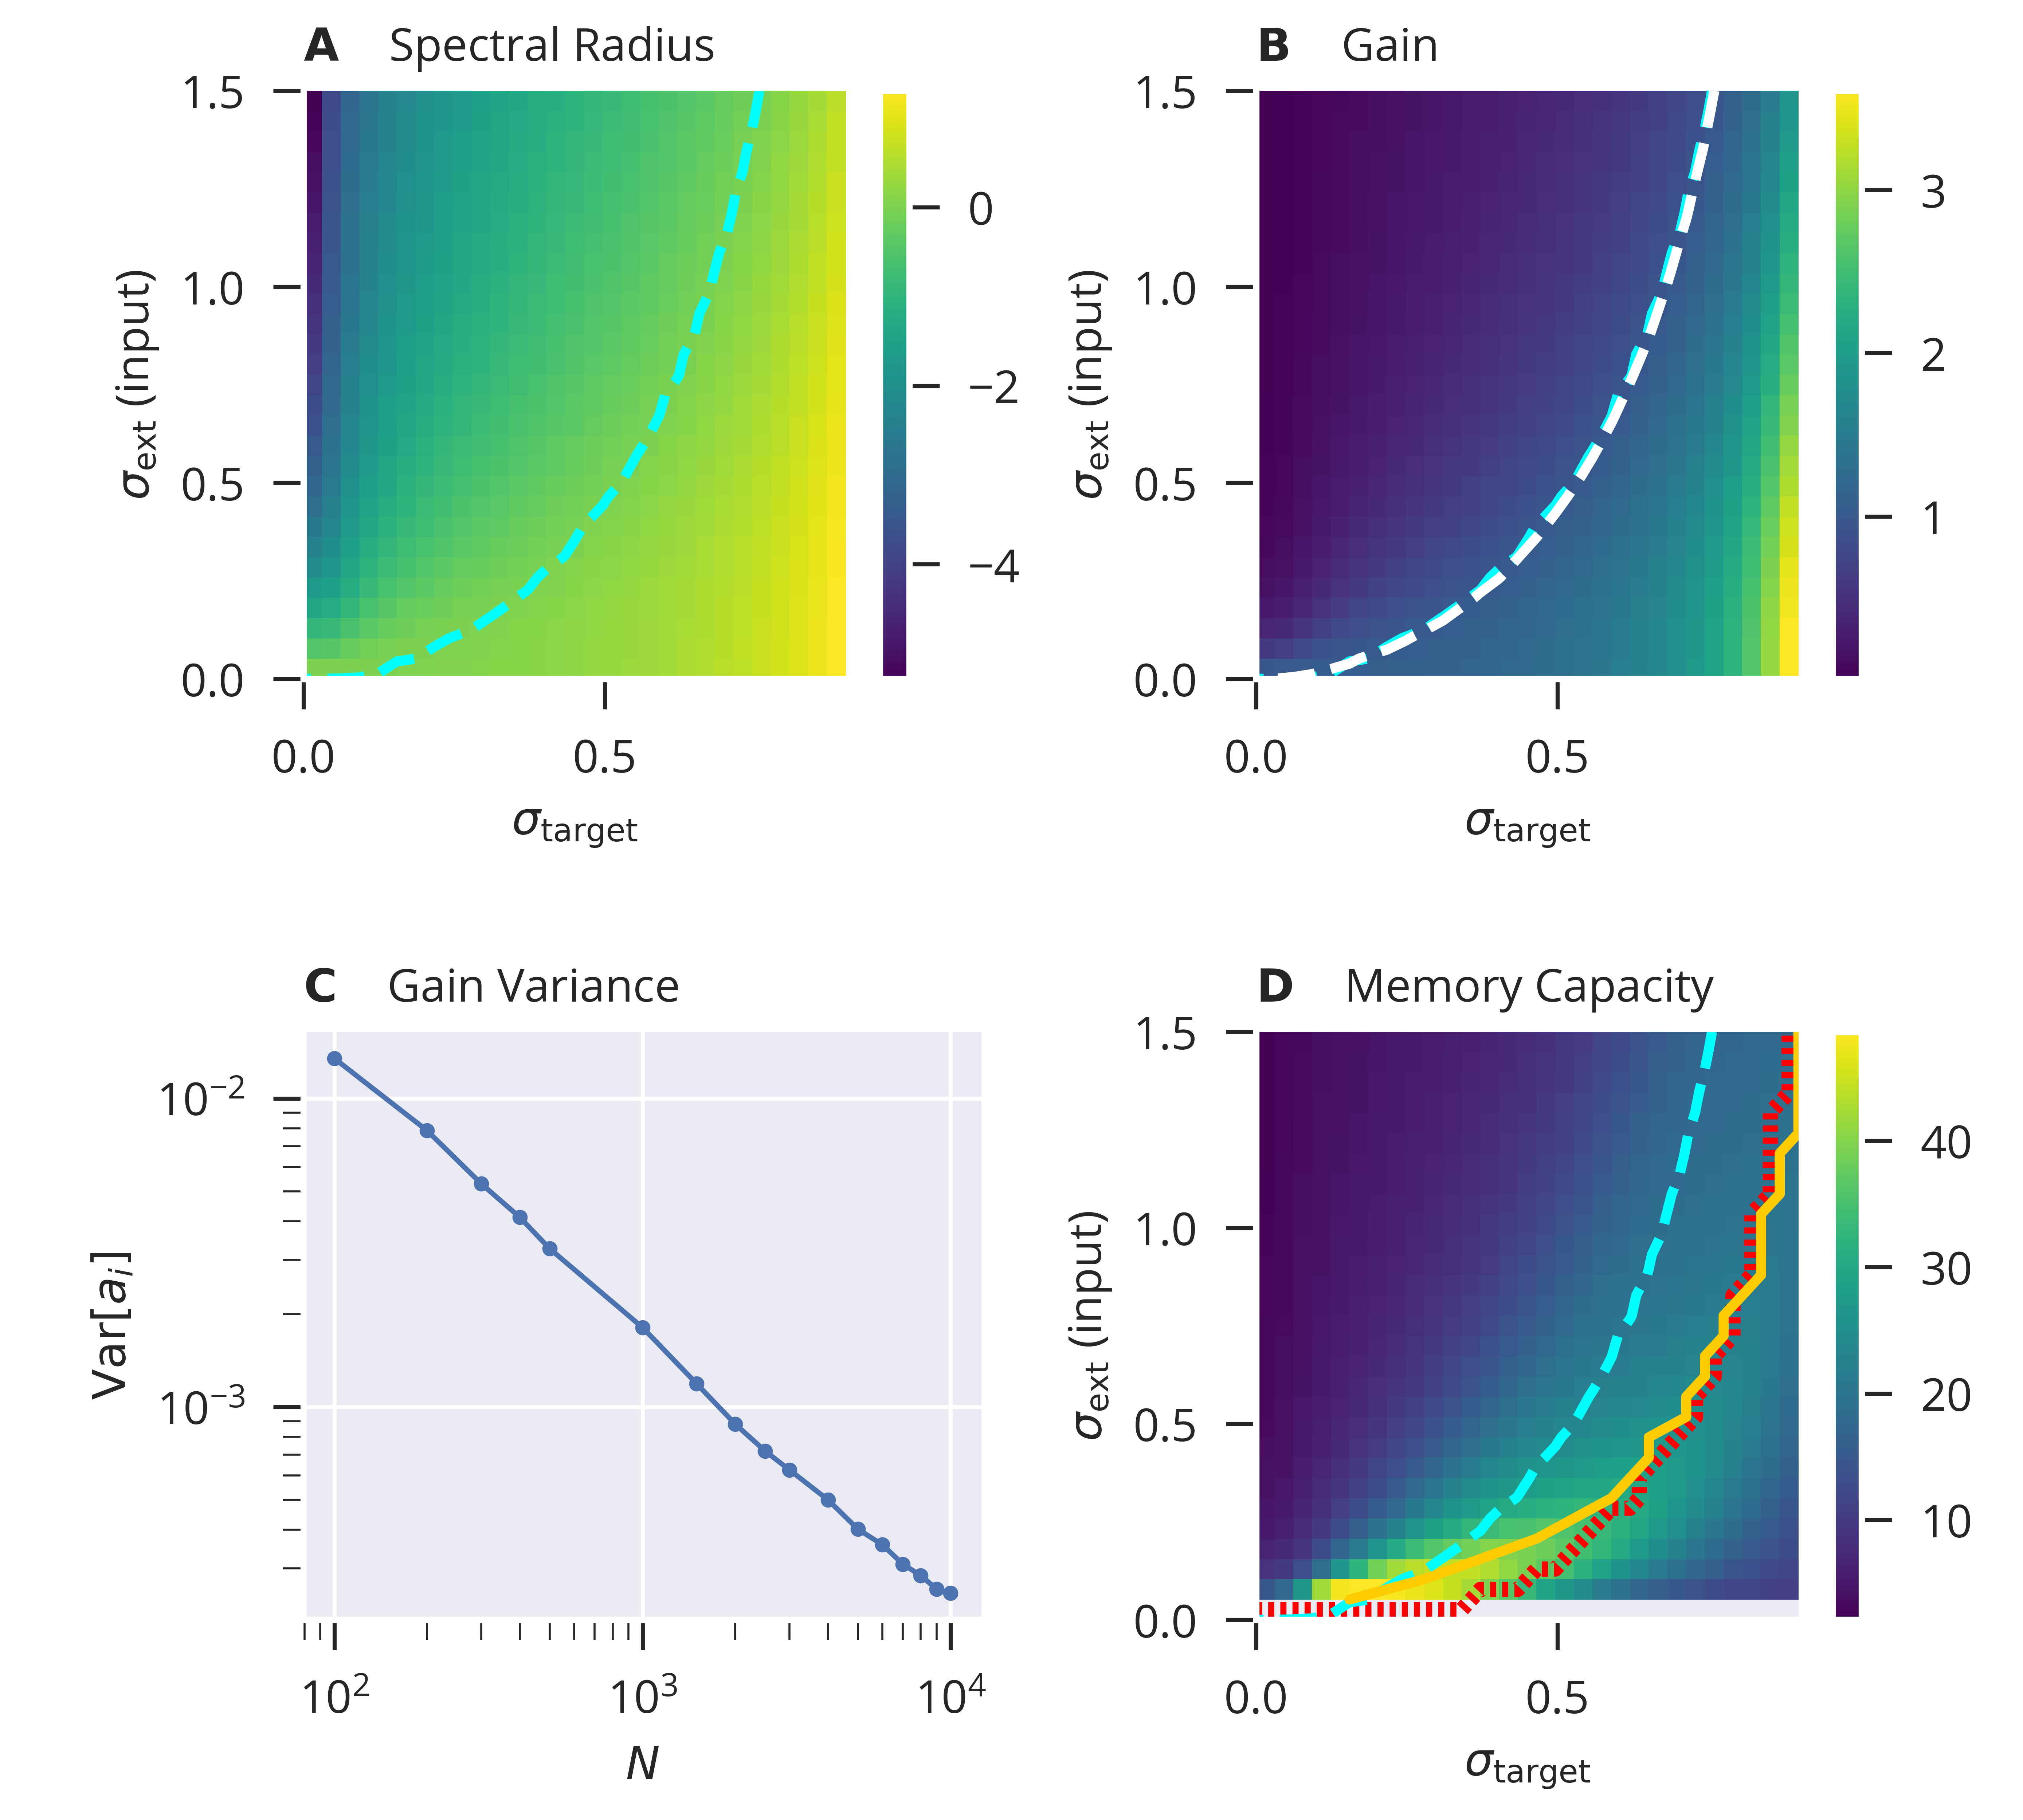
\includegraphics[width=1.0\textwidth]{sigma_target_external.png}
\end{center}
\caption{{\bf Parameter sweep.} For a range of 
$\sigma(\mathrm{target})\!=\!\sigma_{\rm t}$, the target 
for the neuronal activity fluctuations, and
$\sigma(\mathrm{input})\!=\!\sigma_{\rm ext}$, the 
standard deviation of the input.
{\bf A:} On a log-scale, the spectral radius $R$
of the locally rescaled weight matrix (color coded),
as defined by (\ref{R_widehat_W}).
Marked is $\log(R)\!=\!0$ (blue dashed line).
{\bf B:} The population average $\langle a_i\rangle_{\rm P}$ of 
the gain $a_i$ (color coded). Marked is $\langle a_i\rangle_{\rm P}\!=\!1$ 
(white dashed line), which is numerically identical 
to $\log(R)\!=\!0$.
{\bf C:} The variance 
$\mathrm{Var}[a_i]\!=\!\langle(a_i\!-\!\langle a_i\rangle_{\rm P})^2\rangle_{\rm P}$ 
of the gain as a function of system size $N$, as log-log plot.
The falloff is $\sim1/N$.
{\bf D:} The memory capacity (color coded). Highlighted is
the maximal memory capacity for a given $\sigma_{\rm ext}$ 
(orange line, averaged over three trials). Also shown is $\langle a_i\rangle_{\rm P}\!=\!1$ 
(dashed green line) and the onset of the echo state 
property (striped red line). 
}
\label{Fig:sigma_target_external}
\end{figure}
%%%%%%%%%%%%%%%%%%%%%%%%%%%%%%%%%%%%%%%%%%%%

%%%%%%%%%%%%%%%%%%%%%%%%%%%%%%%%%%%%%%%%%%%%
\begin{figure}[t!]
\begin{center}
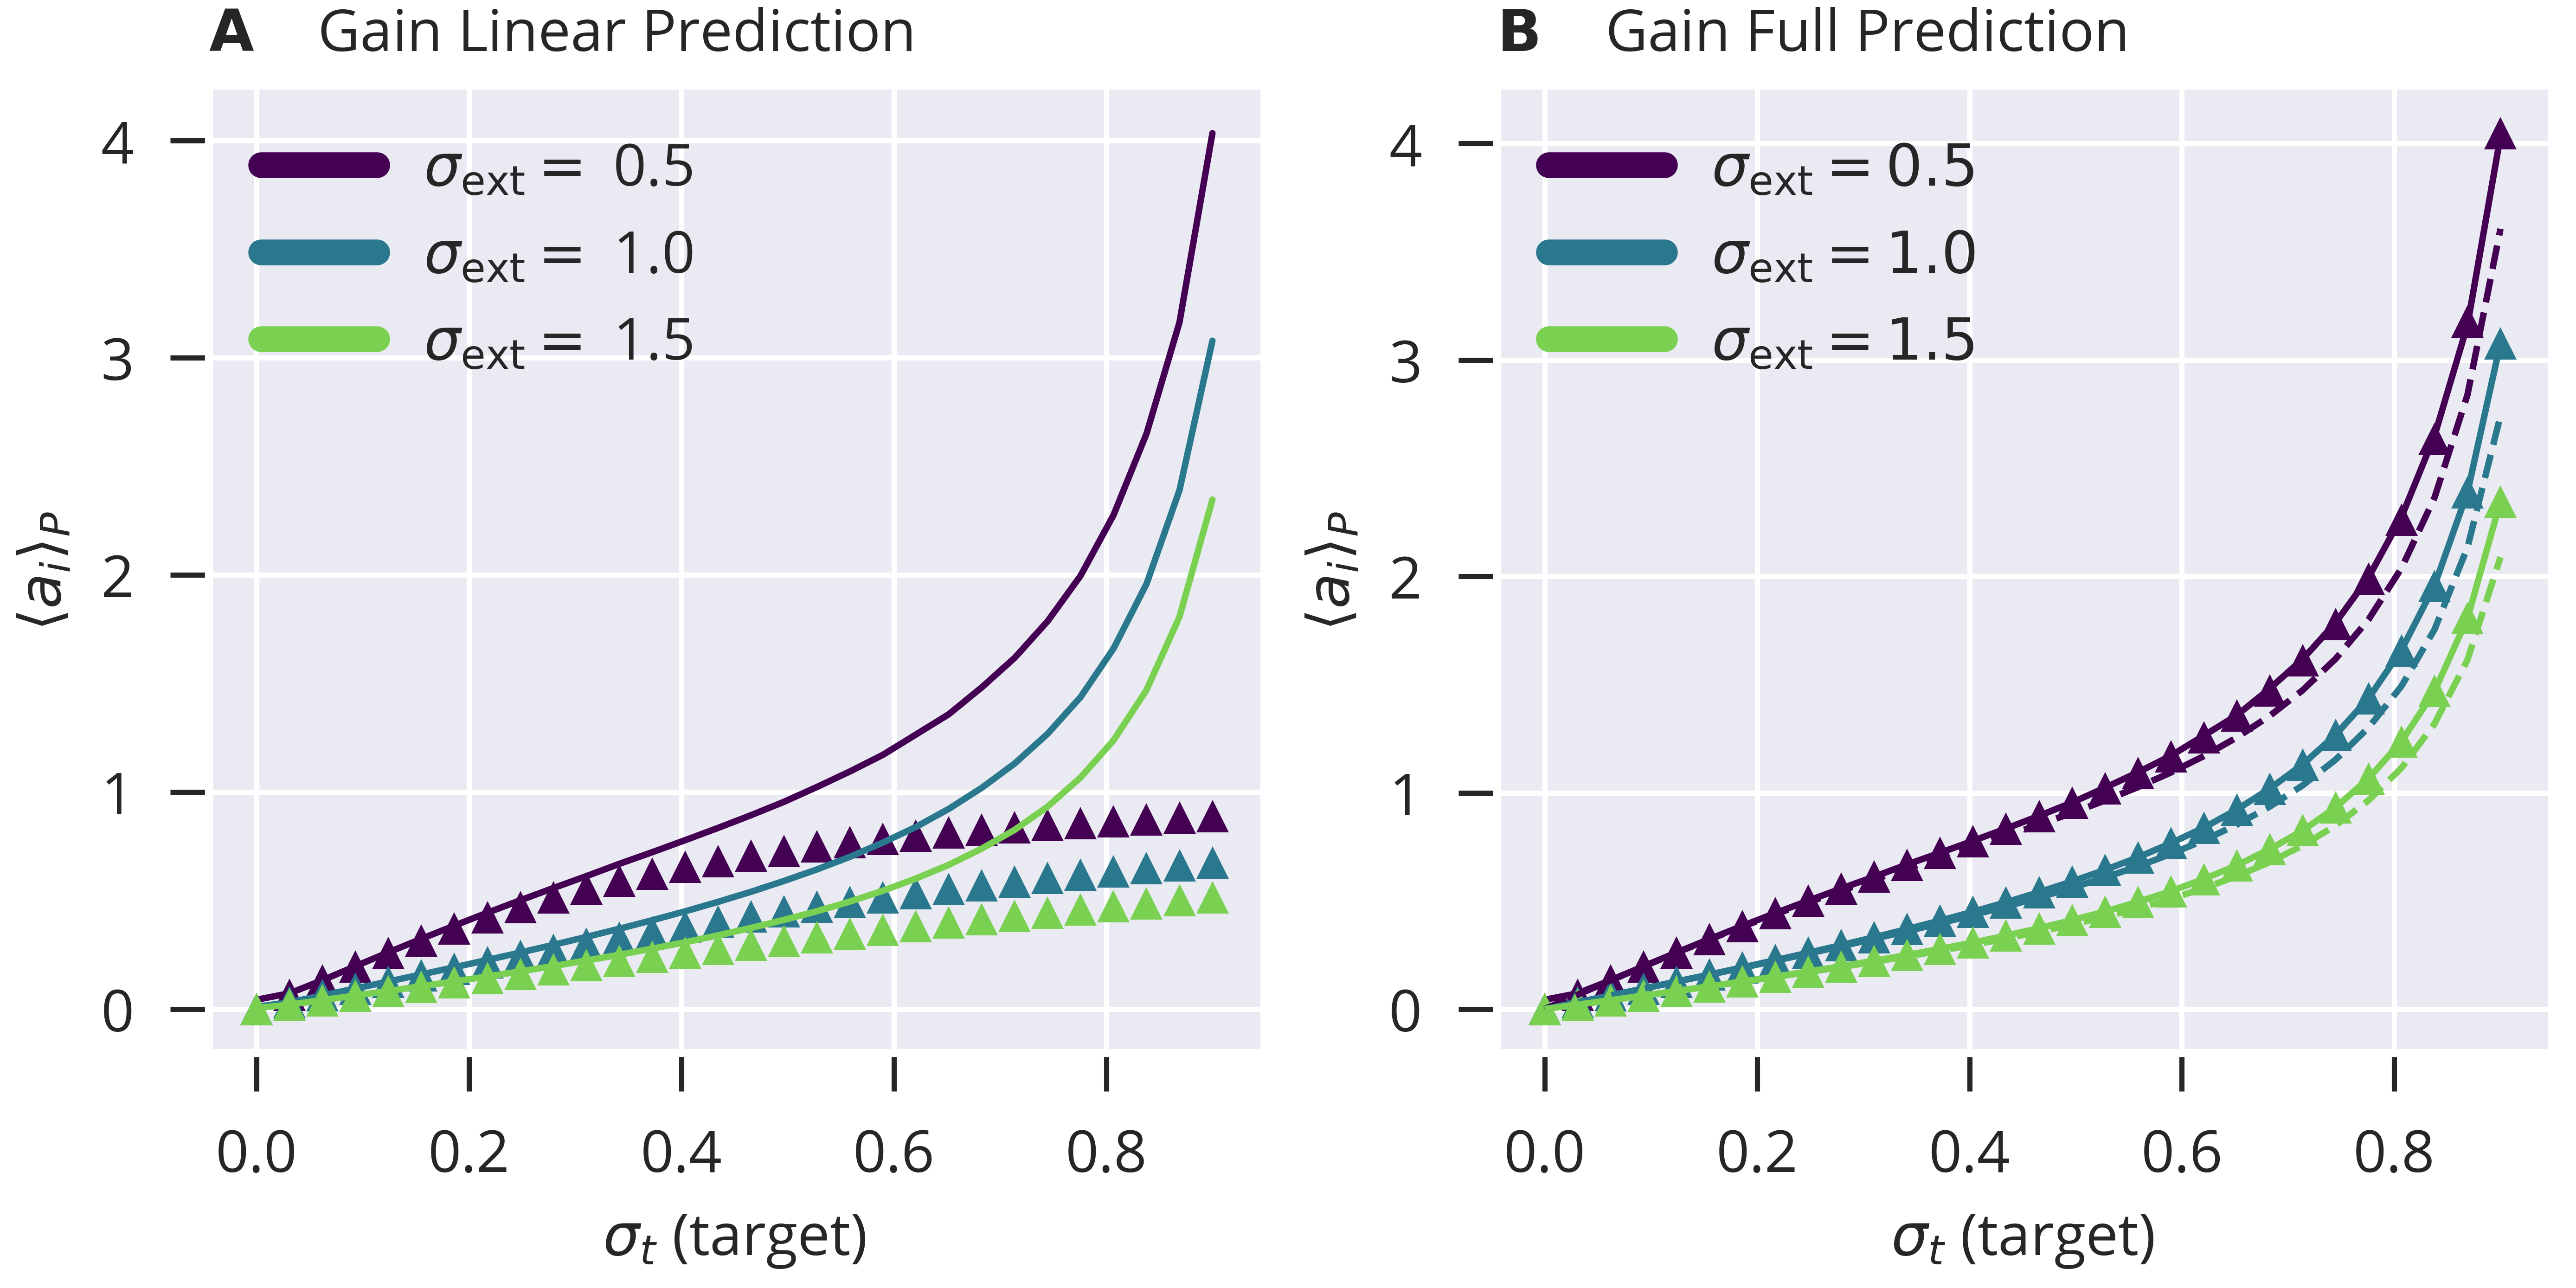
\includegraphics[width=1.0\textwidth]{theory_simulation_1.png}
\end{center}
\caption{{\bf Theory and simulations compared.} 
{\bf A:} Prediction (lines) of and simulation result (triangles) of ${a_i}$. 
{\bf B:} ${a_i}$
from the simulation (triangles) matches the numerically determined solution (lines) of \eqref{self_consistency_z}. Dashed lines are approximations given by \eqref{eq:gain_gaussian_approx}.
}
\label{Fig:theory_simulation_1}
\end{figure}
%%%%%%%%%%%%%%%%%%%%%%%%%%%%%%%%%%%%%%%%%%%%

%%%%%%%%%%%%%%%%%%%%%%%%%%%%%%%%%%%%%%%%%%%%
\begin{figure}[t!]
\begin{center}
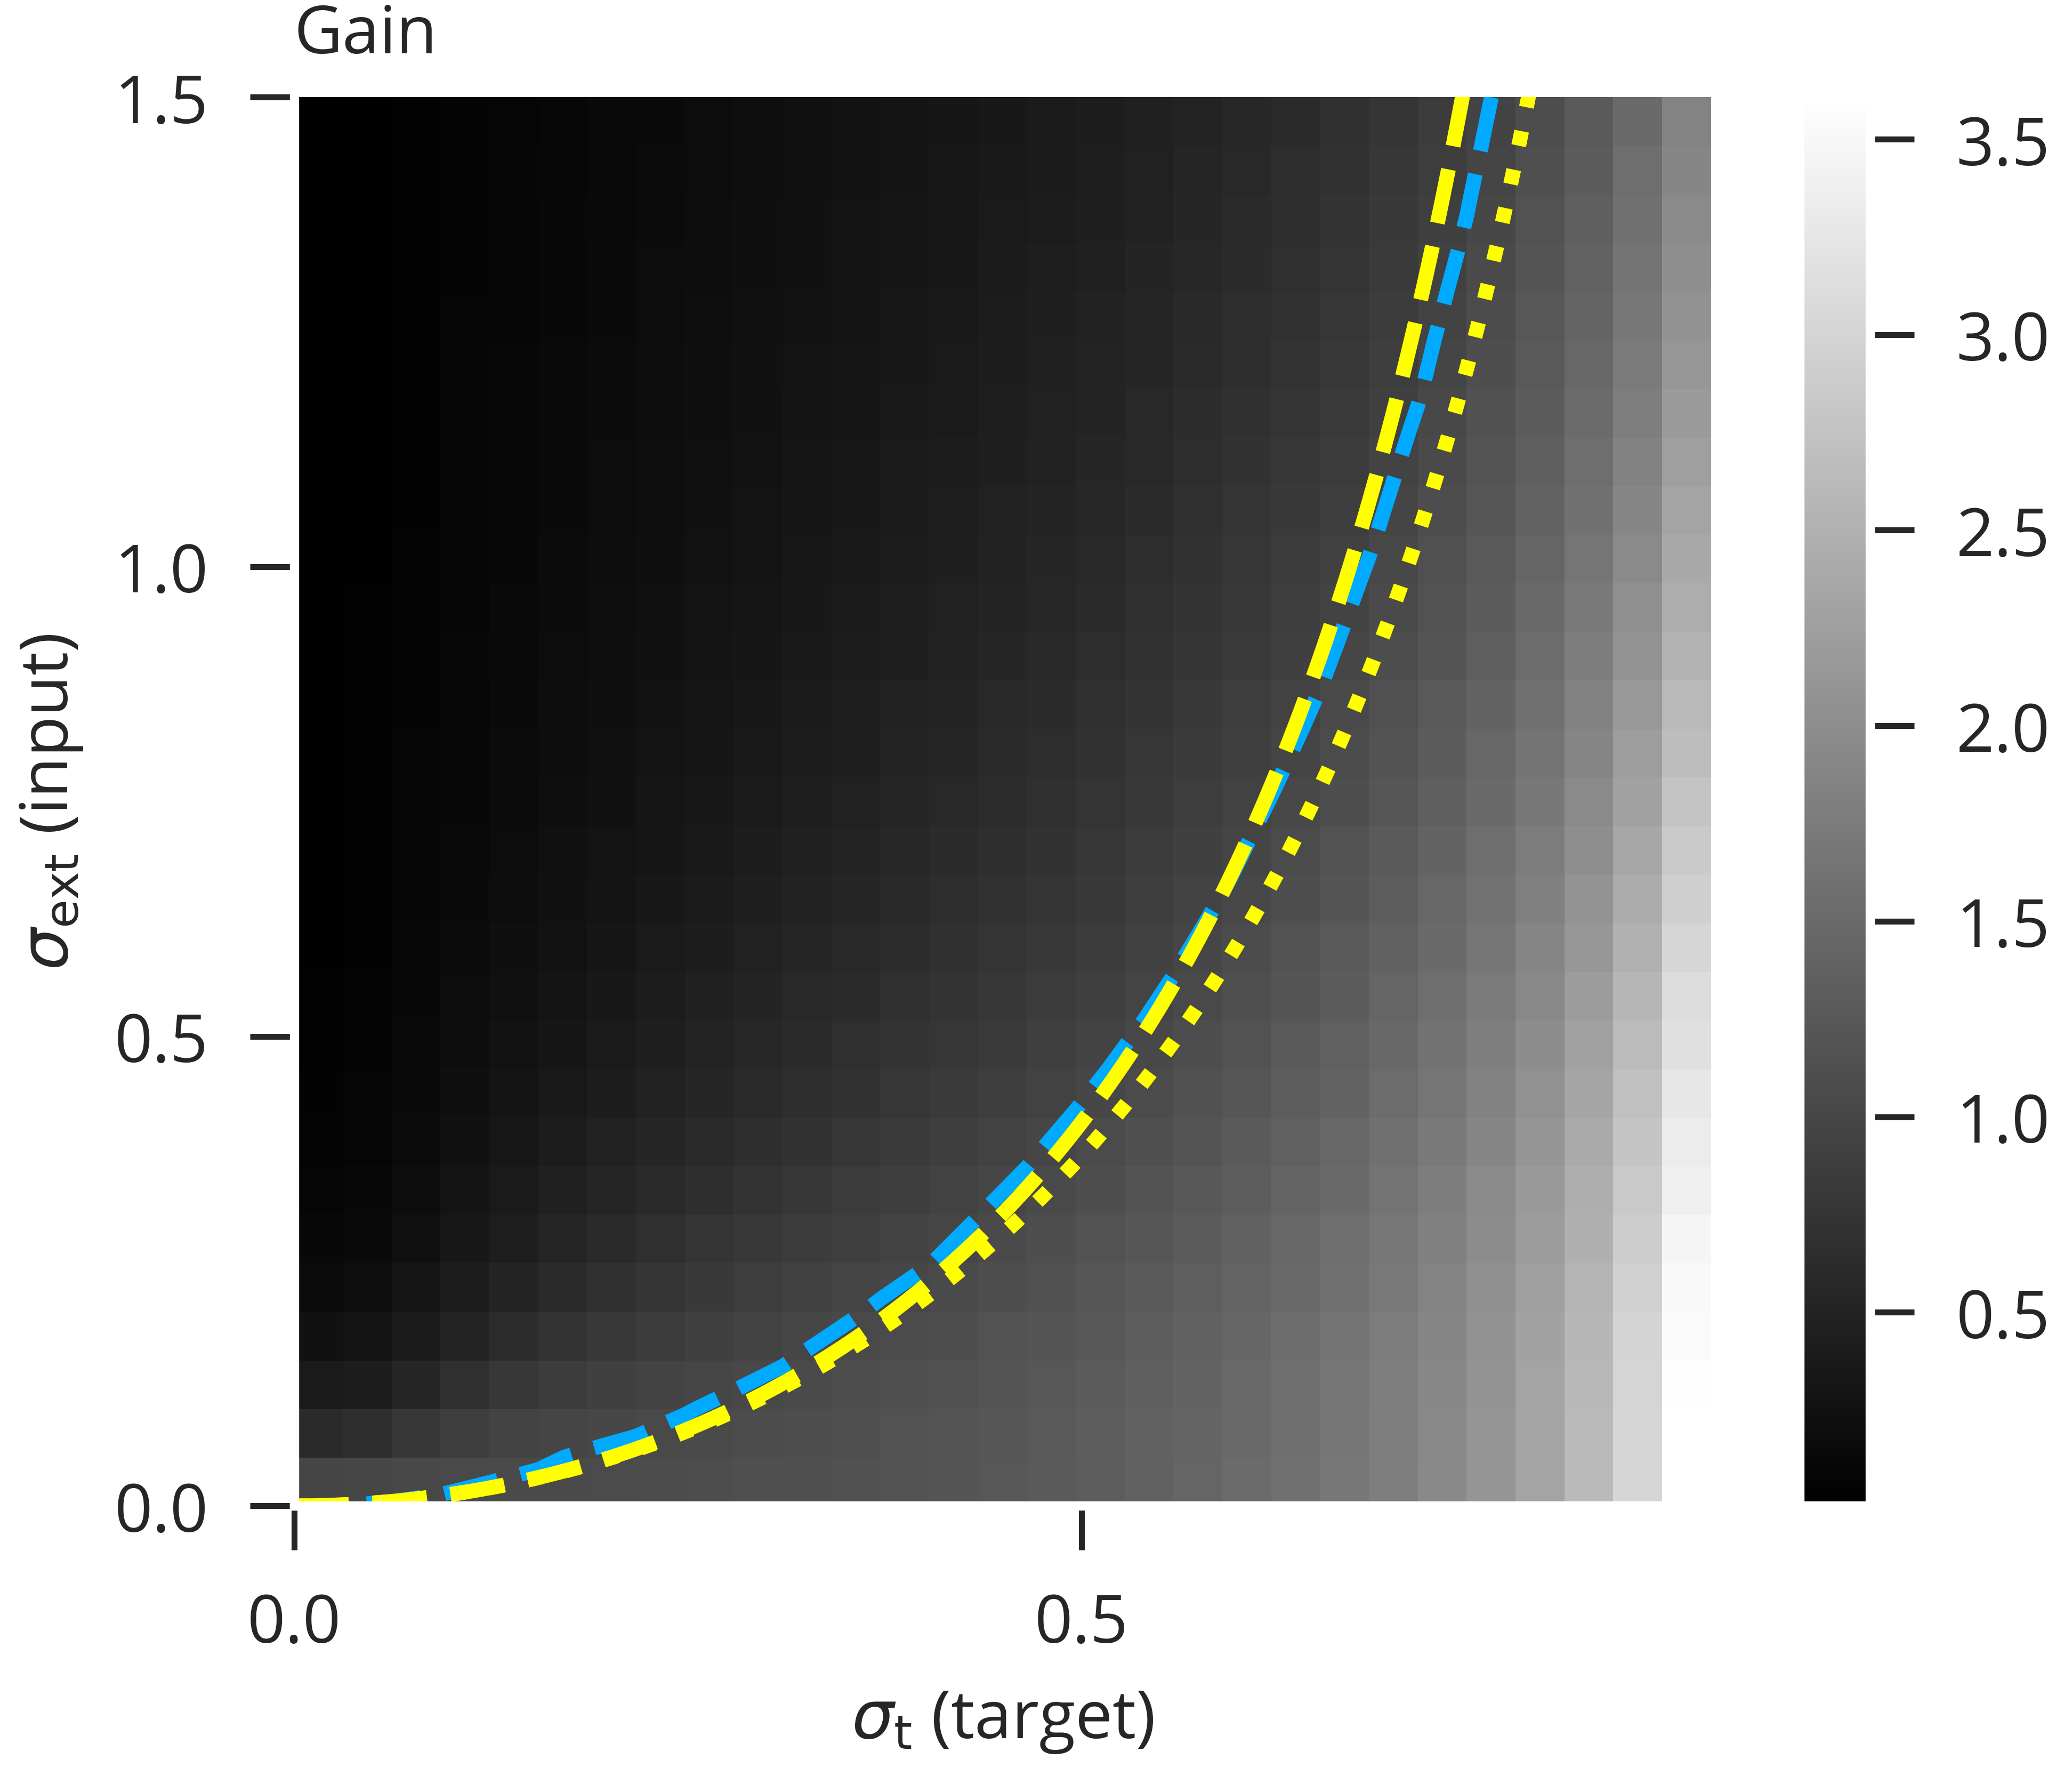
\includegraphics{theory_simulation_2.png}
\end{center}
\caption{{\bf Spectral Radius Transition Approximation} White dashed lines denotes $\langle a_i\rangle_{\rm P}\!=\!1/\sigma_{\rm w}$. Yellow dashed line is given by \eqref{eq:circles_solution_form}, dotted line by \eqref{eq:crit_transition_gaussian_approx}.}
\label{Fig:theory_simulation_2}
\end{figure}
%%%%%%%%%%%%%%%%%%%%%%%%%%%%%%%%%%%%%%%%%%%%

%----------------------------------------
\section{Simulation results}
%----------------------------------------

A typical timeline of network data is presented 
in Figure~\ref{Fig:timeSeries_01}. We used
synchronous updating, as in all simulations.
One observes that the activities $y_i$ decay 
to zero when the external input is turned off, 
which occurs at $t_{\mathrm{off}}=10^5$. 

The characteristic time scale of the evolution of 
the gains $a_i$ shown in Figure~\ref{Fig:timeSeries_01} 
is $1/\epsilon_{\rm b}=0.5\cdot10^4$. For longer times
the individual $a_i$ become quasi stationary, with 
the residual fluctuations being due to the influence 
of the stochastic input on the network activity. The 
spread of the gains is a finite-size effect,
as shown further below. Also included in
Figure~\ref{Fig:timeSeries_01} is a comparison 
between the actual variance of the neural activity
$\sigma^2(y)=\langle (y_i-\bar{y}_i)^2\rangle$,
with the target variance $\sigma_{\rm t}^2$. One finds that the 
adaption rule (\ref{dot_a_b}) does in indeed lead to
$\sigma(y)\to\sigma_{\rm t}$.
For the parameters selected, $\sigma_{\rm t}=0.2$ and 
$\sigma_{\rm ext}=0.1$, spectral radius $R=|\Lambda_{max}|$
adapts to a subcritical value, $R<1$, as shown
in Figure~\ref{Fig:timeSeries_01}, which explains
the decay of the neural activity once the input
is turned off.

For the same parameters as for Figure~\ref{Fig:timeSeries_01},
we present in Fig.~\ref{Fig:timeSeries_02} the time
evolution of the bias $b_i$ and the trailing
averages $\bar{y}_i$, as defined by (\ref{y_trailing}).
The adaption rule (\ref{dot_a_b}) for the bias ensures 
that the the average activity approaches the target, namely
$y_{\rm t}=0$. Note that the stochastic input induces 
barely-visible amplitude fluctuations for the 
thresholds $b_i$.

%----------------------------------------
\section{Theory}
%----------------------------------------

In molecular-field theory one assumes that all
presynpatice neurons are statistical independent.
The optimizing the variance of the neural
activity then consists of solving
%
\begin{equation}
\sigma_{\rm t}^2=\int_{-\infty}^{\infty}
{\rm dx}\tanh^2(ax) N_{\mu,\sigma}(x),
\qquad\quad
\sigma^2=\sigma_{\rm w}^2\sigma_{\rm t}^2+\sigma_{\rm ext}^2\,,
\label{self_consistency_x}
\end{equation}
%
where the distribution $N_{\mu,\sigma}(x)$ is 
of the membrane potential $x$ is a Gaussian,
see (\ref{Gaussian}), with mean $\mu=0$
and variance $\sigma^2$.
A variable transformation $ax=z$ leads to
%
\begin{equation}
\sigma_{\rm t}^2=\int_{-\infty}^{\infty}
{\rm dz}\tanh^2(z) \frac{1}{\sqrt{2\pi\sigma_{\rm a}^2}}
\mathrm{e}^{-z^2/2\sigma_{\rm a}^2}
\qquad\quad
\sigma_{\rm a}^2=a^2\big(\sigma_{\rm w}^2\sigma_{\rm t}^2+\sigma_{\rm ext}^2\big)\,,
\label{self_consistency_z}
\end{equation}
%
where the renormalized variance $\sigma_{\rm a}^2$ can
be written as
%
\begin{equation}
\sigma_{\rm a}^2=
a^2\sigma_{\rm w}^2\big(\sigma_{\rm t}^2+\sigma_{\rm ext}^2/\sigma_{\rm w}^2\big)\,.
\label{sigma_a_renormalized}
\end{equation}
%
The gain $a$ is adapted such that (\ref{self_consistency_z})
is fulfilled, defining a 2d-manifold in the $(\sigma_{\rm t},\sigma_{\rm ext},a)$ space. The relation (\ref{sigma_a_renormalized}) shows furthermore
that the solution of (\ref{self_consistency_z}) depends on the ratio $\sigma_{\rm ext}/\sigma_{\rm w}$, which measures the relevance of the external driving with respect the recurrent synaptic connections. For convenience, we thus introduce $\sigma^\prime_{\rm ext} \equiv \sigma_{\rm ext}/\sigma_{\rm w}$

\subsection{Polynomial Approximation}
Approximating the transfer function with
$\tanh^2(z)\approx z^2-2 z^4/3$ one may carry out
the Gaussian integral occurring on the right-hand
side of (\ref{self_consistency_z}), with the result
%
%\begin{equation}
%\sigma_{\rm t}^2 +\frac{\sigma_{\rm ext}^4}{\sigma_{\rm w}^4}
%+2\frac{\sigma_{\rm t}^2\sigma_{\rm ext}^2}{\sigma_{\rm w}^2}
%=\frac{\sigma_{\rm ext}^2}{2\sigma_{\rm w}^2},
%\qquad\quad a=\frac{1}{\sigma_{\rm w}}\,.
%\label{analytic_solution}
%\end{equation}

\begin{equation}
\sigma_{\rm t}^2 \approx a^2 \sigma^2_{\rm w}\left( \sigma^2_{\rm t} + {\sigma^\prime}^2_{\rm ext} \right) - 2a^4  \sigma^4_{\rm w} \left(\sigma^2_{\rm t} + {\sigma^\prime}^2_{\rm ext} \right)^2 = \sigma^2_{\rm a} - 2\sigma^4_{\rm a} \label{eq:sec_order_approx_consistency}
\end{equation}

We can use this equation to find an approximate solution of the critical transition of the autonomous network, denoted by the line in Fig.~\ref{Fig:sigma_target_external}. This transition is generally given by $a = 1/\sigma_{\rm w}$. This leads to the equation

\begin{equation}
\left[\left(\sigma_{\rm ext} - \frac{1}{\sqrt{8}}\right)^2 + \sigma_{\rm t}^2 - \frac{1}{8}\right]\left[\left(\sigma_{\rm ext} + \frac{1}{\sqrt{8}}\right)^2 + \sigma_{\rm t}^2 - \frac{1}{8}\right] = 0 \; . \label{eq:circles_solution_form}
\end{equation}

From this form we can see that the solution set consists of two circles with radius $1/\sqrt{8}$ in the $\sigma_{\rm t}$, $\sigma_{\rm ext}$ space, centered around $\sigma_{\rm t} = 0$, $\sigma_{\rm ext} = \pm 1/\sqrt{8}$. Fig.~\ref{Fig:theory_simulation_2} shows a comparison between this approximation (yellow line) and the simulation (white line).

\subsection{Gaussian Approximation}
A polynomial approximation of $\tanh^2$ to fourth order captures the right behavior close to the origin, but does not account for the fact that $\tanh^2$ converges to $1$ for large absolute values of the membrane potential. Alternatively, an approximation with the correct scaling to second order as well as the right convergence is
\begin{equation}
	\tanh^2(x) \approx 1 - \exp\left(-x^2 \right) \; .
\end{equation}

Using this approximation in \eqref{self_consistency_z} and solving the integral yields
\begin{equation}
	\sigma^2_{\rm t} = 1 - \sqrt{1+2a^2\sigma^2_{\rm w}\left( \sigma^2_{\rm t} + {\sigma^\prime}^2_{\rm ext} \right)} \; . \label{eq:gaussian_approx}
\end{equation}
Solving this equation for $a$ gives
\begin{equation}
	a = \sigma^{-1}_{\rm w} \sqrt{\frac{1-\left(1-\sigma^2_{\rm t}\right)^2}{2\left(1-\sigma^2_{\rm t}\right)^2\left(\sigma^2_{\rm t} + {\sigma^\prime}^2_{\rm ext} \right)}} \; . \label{eq:gain_gaussian_approx}
\end{equation}
As shown in Fig.~\ref{Fig:theory_simulation_1}B, this approximation matches the exact solution to a high accuracy.

As in the previous section, we can also derive an approximation for the critical transition from \eqref{eq:gaussian_approx}, which is given by
\begin{equation}
	\sigma^\prime_{\rm ext} = \sqrt{\frac{1}{2\left(1-\sigma^2_{\rm t}\right)^2} -\sigma^2_{\rm t} - \frac{1}{2}} \; . \label{eq:crit_transition_gaussian_approx}
\end{equation} 
See Fig.~\ref{Fig:theory_simulation_2} for a comparison.


\subsection{ESP Transition}
The so called \textit{echo state property} was formally described in \cite{Jaeger_2001}. In short, it states that there exists at least one left-infinity input sequence for which the state sequence of the recurrent network is uniquely determined by this input sequence. In particular, this means that the effect of different initial conditions of the recurrent network will decay. The transition shown in Fig.~\ref{Fig:sigma_target_external}D by the red striped line was determined using this effect by initializing two copies of a network with a small perturbation in the initial conditions and then observing the euclidean distance between both network states while feeding in the same quenched random input.

Assuming that the perturbation is sufficiently small, we modeled the evolution of this initial offset $\delta_i$ by a linear approximation:

\begin{align}
	\delta_i(t+1) &\approx a y_i^\prime(t+1) \sum_j w_{ij} \delta_j(t) \label{eq:esp_dist_evolution1} \\
	&= a \left( 1 - \tanh\left( a \left( x_i(t+1) - b_i\right)\right)^2\right) \sum_j w_{ij} \delta_j(t) \label{eq:esp_dist_evolution2}
\end{align}

Furthermore, we make the assumption that the trajectory of the recurrent network state is sampling from phase space in a quasi-random way. More specifically, we again assume that neural activity is essentially uncorrelated in time and across the population, which was also the assumption made for \eqref{self_consistency_x}. With respect to simplifying \eqref{eq:esp_dist_evolution2}, this assumption allows us to interpret $\left( 1 - \tanh\left( a \left( x_i - b_i\right)\right)^2\right)$ as an independent random vector drawn from $\left( 1 - \tanh\left( a x \right)^2\right)$, where $x$ is Gaussian distributed with the usual $\mu_{\rm x} = 0$, $\sigma^2_{\rm x} = \sigma^2_{\rm w}\sigma^2_{\rm t} + \sigma^2_{\rm ext}$.

We can write \eqref{eq:esp_dist_evolution1} as
\begin{align}
	\delta_i(t+1) &= \sum_j A_{ij}(t+1) \delta_j(t) \\
	A_{ij} &\defeq a \left( 1 - \tanh\left( a \left( x_i(t+1) - b_i\right)\right)^2\right) w_{ij}
\end{align}

To determine the long term evolution of $\norm{\delta}(t)$, we would like to evaluate the average growth factor
\begin{equation}
	\gamma = \left\langle \frac{\norm{\delta(t+1)}}{\norm{\delta(t)}} \right\rangle_{\rm t} \; \label{eq:av_growth_rate}
\end{equation}
Since \eqref{eq:esp_dist_evolution1} is a linear system, we can rescale terms in \eqref{eq:av_growth_rate} such that the denominator becomes one and only evaluate the change in length for each time step:

\begin{align}
	\gamma &= \left\langle \norm{\Delta (t)} \right\rangle_t \label{eq:rescale_growth1} \\
	\Delta (t) &\defeq \widehat{A}(t) \delta^\prime (t-1) = \widehat{A}(t) \delta(t-1) / \norm{\delta(t-1)}   \label{eq:rescale_growth2}
\end{align}
 
In principle, $\delta (t)$ and thus also $\Delta (t)$ are not independent in time, since they are iteratively generated. However, since all $A(t)$ are assumed to be independent, we can also regard $\delta (t)$ as statistically independent in time (THIS IS VERY HAND-WAVY, BUT I'M NOT SURE HOW TO FURTHER JUSTIFY THIS).

We express \eqref{eq:rescale_growth1} as
\begin{equation}
	\gamma = \left\langle \sqrt{\sum_i \left( \sum_j A_{ij}(t+1) \delta^\prime_j(t) \right)^2} \right\rangle_{\rm t} \; .
\end{equation}

For large $N$, the inner sum follows a Gaussian distribution with $\mu_{\sum} = N \mu_A \mu_{\delta^\prime}$ and $\sigma^2_{\sum} = N \sigma^2_A \sigma^2_{\delta^\prime}$. Since $\mu_A = 0$, we have

\begin{align}
	\gamma &= \left\langle \sqrt{\sum_i  X^2_i(t)} \right\rangle_{\rm t} \label{eq:Chi_Squ1} \\
	&= \sigma_{\sum} \left\langle \sqrt{\sum_i X^2_i(t)} \right\rangle_{\rm t} \label{eq:Chi_Squ2} 
\end{align}
where $X$ follows a standard Gaussian distribution. The remaining sum obeys a Chi-squared distribution which, for large N, again follows a Gaussian distribution with mean $N$ and variance $2N$, which allows us to ignore fluctuation around the mean for large $N$:
\begin{align}
	\gamma &= \sigma_{\sum} \left\langle \sqrt{ \sqrt{2N} X(t) + N }  \right\rangle_{\rm t} \\
	&\approx \sigma_{\sum} \sqrt{N} \\
	& =  N \sigma_A \sigma_{\delta^\prime}
\end{align}
The empirical variance of $\delta^\prime$ is
\begin{equation}
	\sigma^2_{\delta^\prime} = \frac{1}{N T} \sum_{i,t} {\delta^\prime_i}(t)^2 - \mu_{\delta^\prime}^2 \; .
\end{equation}
For all $t$, the sum over $i$ is one by definition. $\delta^\prime(t)$ is a sequence of points on a $N$-dimensional unit sphere. A non-zero mean value would imply that there is a ��preferred direction" in the sequence distribution. However, since we have assumed that the mapping $\widehat{A}(t)$ is randomly drawn from statistics that are the same for each coordinate (symmetric under exchange of coordinates), this mapping will generate a distribution with the same symmetrical property (VERY BOLD STATEMENT), thus giving zero mean.

We now find for $\gamma$
\begin{align}
	\gamma &= \sqrt{N}\sigma_A \\
	&= \sqrt{N} a \sqrt{ \mathrm{E}[w^2]\mathrm{E}[{y^\prime}^2] - \mathrm{E}[w]^2\mathrm{E}[{y^\prime}]^2 } \\
	&= \sqrt{N} a \sqrt{\mathrm{E}[w^2]\mathrm{E}[{y^\prime}^2] } \\
	&= a \sigma_{\rm w} \sqrt{\mathrm{E}[{y^\prime}^2]} \\
	&= a \sigma_{\rm w} \sqrt{\int_{-\infty}^{\infty} {\rm dx} \left(1 - \tanh^2\left( a x \right) \right)^2 N_{\mu=0,\sigma}(x)},
		\qquad
		\sigma^2=\sigma_{\rm w}^2\left(\sigma_{\rm t}^2+{\sigma^\prime_{\rm ext}}^2 \right) \; . \label{eq:esp_trans_exact}
\end{align}
Similar to the approximation used to find an explicit equation for $a(\sigma_{\rm w},\sigma^\prime_{\rm ext})$, we use $\left(1 - \tanh^2\left( a x \right) \right)^2 \approx \exp\left( -2a^2x^2 \right)$, leading to
\begin{equation}
	\gamma \approx a \sigma_{\rm w} \left( 1 + 4a^2\sigma^2 \right)^{-1/4} \; . \label{eq:esp_trans_approx}
\end{equation}



\begin{figure}
	\centering
	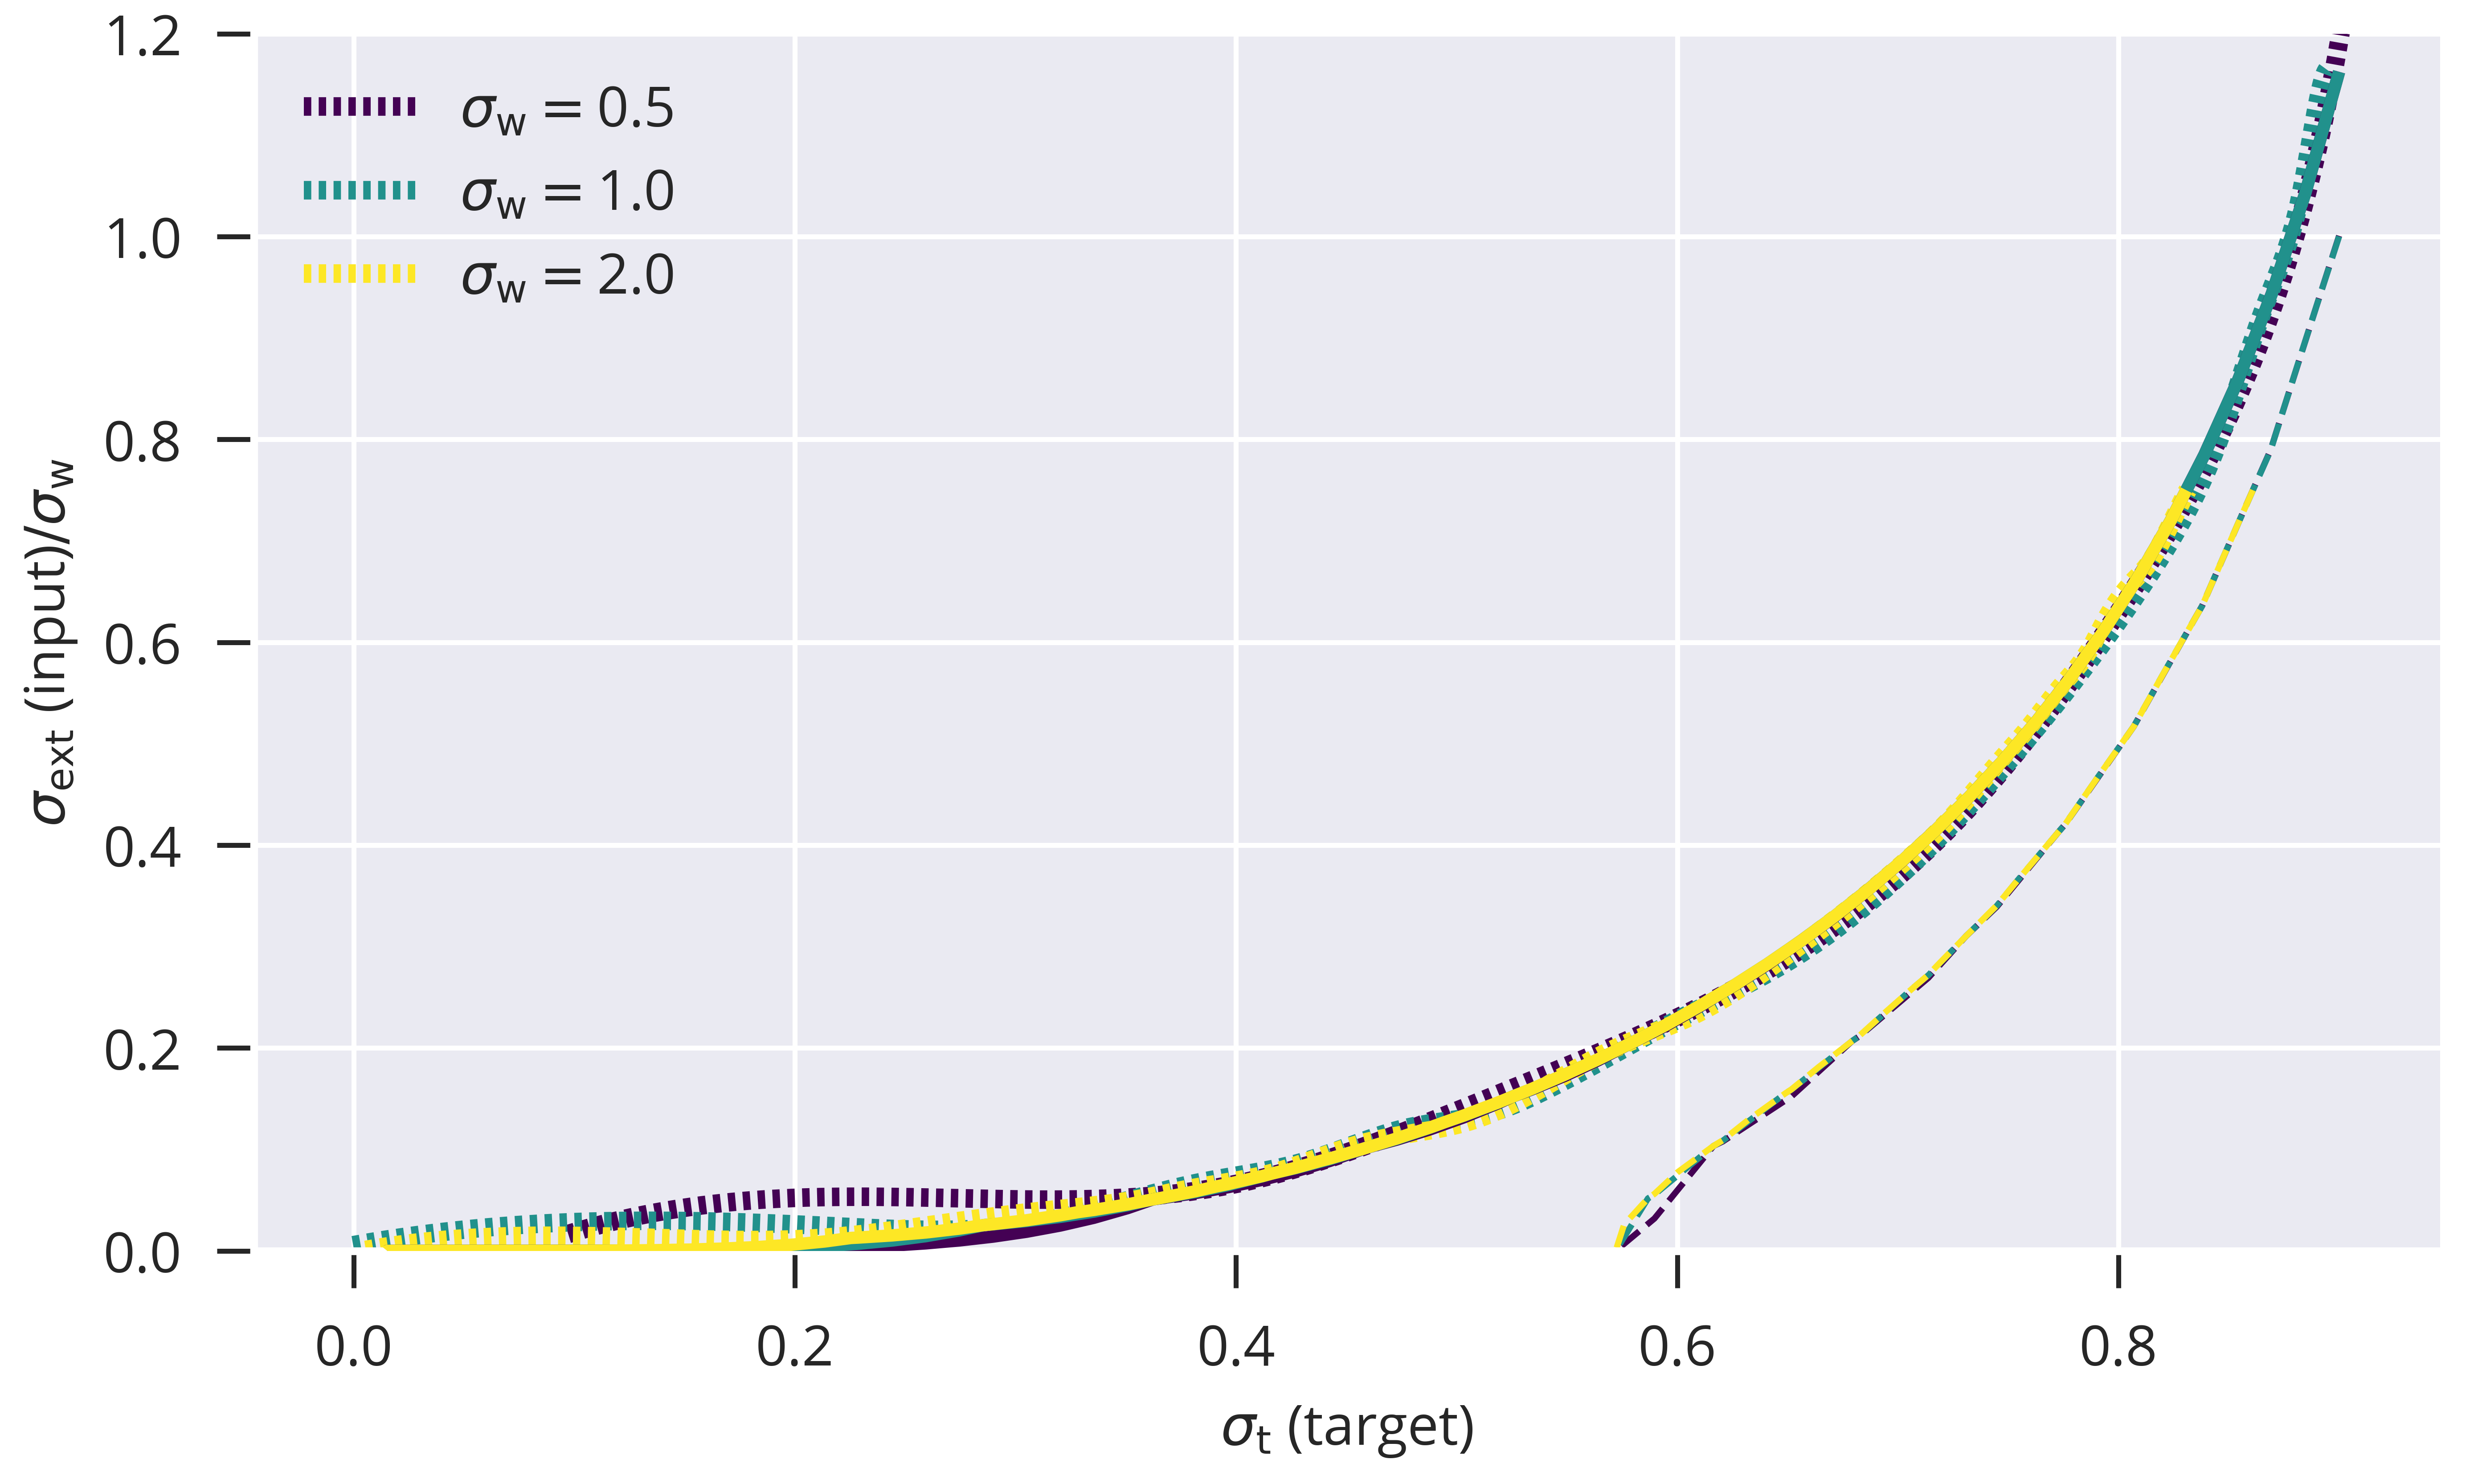
\includegraphics[width=\textwidth]{esp_prediction.png}
	\caption{Striped lines: ESP-transition for full simulations. Dashed lines: approximation given by \eqref{eq:esp_trans_approx}. Full lines: Exact solution defined by \eqref{eq:esp_trans_exact} and \eqref{self_consistency_x}.}
\end{figure}







 

%----------------------------------------
\section*{Conclusion}
%----------------------------------------
We have illustrated the basic format to the manuscript that you consider to
submit to Neural Computation. We hope this is helpful to the authors.

%----------------------------------------
\subsection*{Acknowledgments}
%----------------------------------------
The people you want to acknowledge. For this document, we appreciate J�rg
L�cke, author of an accepted paper who generously allowed us to use his
template.

\section*{Appendix}
You should put the details that are not required in the main body into this Appendix.

%%%%%%%%%%%%%%%%%%%%%%%%%%%%%%%%%%%%%%%%%%%%%%%%%%%%%%%
\bibliographystyle{humannat}
\bibliography{schubert_echo}
%%%%%%%%%%%%%%%%%%%%%%%%%%%%%%%%%%%%%%%%%%%%%%%%%%%%%%%

\end{document}
